\documentclass{beamer}
%\usepackage{longtable}
%\usepackage{graphicx}
%\usepackage{afterpage}
\usepackage[T1]{fontenc}
\usepackage[utf8]{inputenc}
\usepackage{appendixnumberbeamer}

%\usefonttheme{structuresmallcapsserif}
\usefonttheme{structurebold}
\usetheme{AnnArbor}
%\usetheme{Malmoe}
%\usetheme{Dresden} 
 
%Information to be included in the title page:
\title{Računalna statistička analiza jezika religijskih rasprava na internetskim forumima}
\author{Autor: Josip Torić \\ Mentor: izv. prof. dr. sc. Jan Šnajder}
\date{11. srpnja 2018.}
\institute{Fakultet elektrotehnike i računarstva, Sveučilište u Zagrebu}
 
%\logo{\includegraphics[height=1.5cm]{lion-logo.png}}
 
\begin{document}
 
\frame{\titlepage}

\begin{frame}
\frametitle{Uvod}



Religija je sastavni dio života svakog čovjeka, a pri tome je uopće ne bitno je li čovjek religiozan ili nije.
\bigskip

Cilj rada je analizirati tekstove religijskih rasprava uz pomoć statističke analize.
\bigskip

\end{frame}


 
\begin{frame}
\begin{center}
\Huge Statistička analiza jezika
\end{center}

\end{frame}



\begin{frame}
\frametitle{Deskriptivna statistička analiza} 
Deskriptivna statistička analiza bavi se mjerama centralne tendencije i mjerama rasipanja.
\bigskip


Najvažnije mjere centralne tendencije su:
\begin{itemize}
 \item aritmetička sredina
 \item medijan
 \item mod
\end{itemize}

\end{frame}

\begin{frame}
\frametitle{Odnos mjera centralne tendencije}
\begin{figure}[]
	\centering
	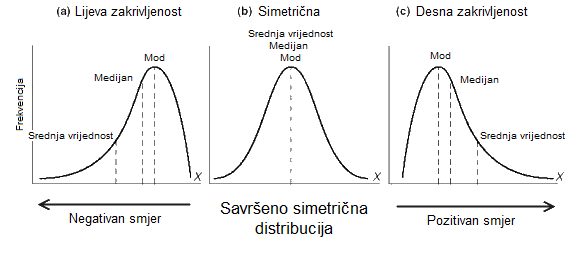
\includegraphics[width=9cm]{img/meanmedianmode.png}
	\caption{Odnos aritmetičke sredine, medijana i mode ovisno o zakrivljenosti distribucije.}
	\label{fig:meanmedmode}
\end{figure}

\end{frame}

\begin{frame}
\frametitle{Mjere rasipanja}
Najvažnije mjere rasipanja su:
\begin{itemize}
 \item rang
 \item interkvartilni rang
 \item varijanca
 \item standardna devijacija
 \item koeficijent varijacije
\end{itemize}
\end{frame}


\begin{frame}
\frametitle{Vizualizacija standardne devijacije}
\bigskip
\begin{figure}[]
	\centering
	\small
	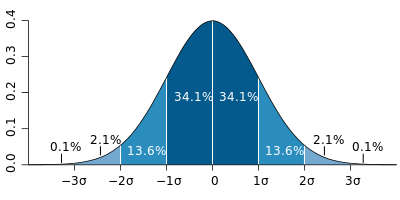
\includegraphics[width=9cm]{img/deviation.png}
	\caption{Standardna devijacija u normalnoj distribuciji.}
	\label{fig:deviation}
\end{figure}
\bigskip
\end{frame}

\begin{frame}
\frametitle{Inferencijalna statistička analiza}
Inferencijalna analiza odnosi se na provjeravanje postavljenih hipoteza uz pomoć statističkih testova.

\bigskip
Inferencijalna statistička analiza se provodi na sljedeći način:

\begin{itemize}
 \item Postavljanje hipoteza
 \item Odabiranje testne statistike
 \item Odabiranje nivoa značajnosti $\alpha$
 \item Izračunavanje vrijednosti statistike i usporedba s $\alpha$
\end{itemize}
\end{frame}

\begin{frame}
\frametitle{Eksplorativna statistička analiza}
Eksplorativna statistička analiza za razliku od deskriptivne i inferencijalne analize ne fokusira se na osnovne podatke o podacima i testiranje hipoteza.
\bigskip

Cilj eksplorativne statistička analiza je istražiti podatke bez definiranih ciljeva u početku te pokušati formulirati sasvim nove hipoteze o podatcima.
\end{frame}

\begin{frame}
\frametitle{Proces obrade podataka}

\begin{figure}[]
	\centering
	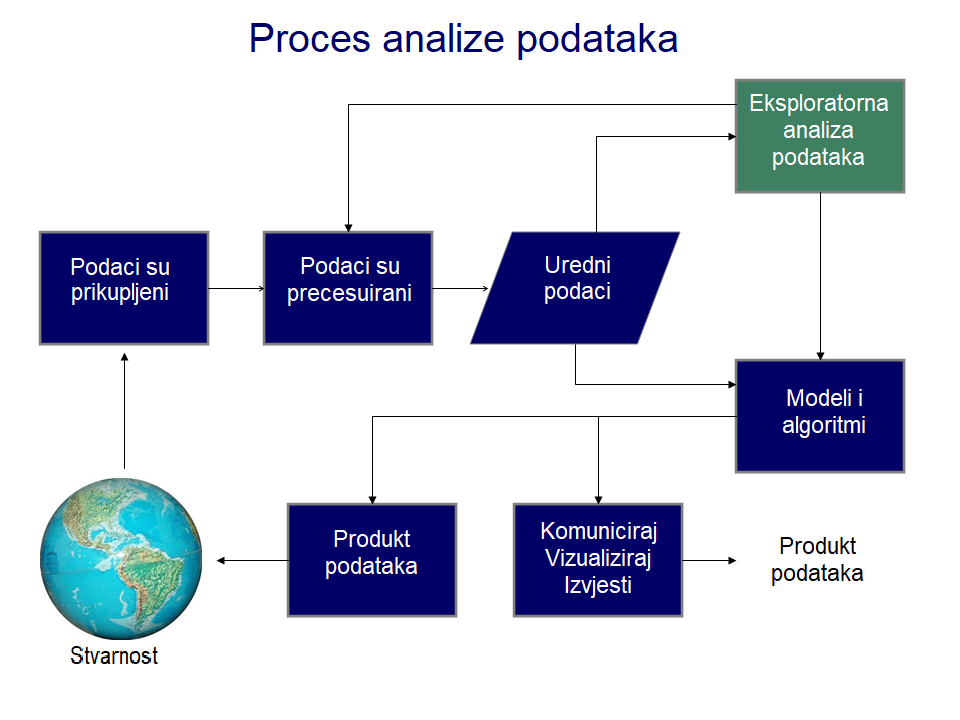
\includegraphics[width=8cm]{img/eda.png}
	\caption{Proces obrade podataka u eksplorativnoj statističkoj analizi.}
	\label{fig:eda}
\end{figure}

\end{frame}

\begin{frame}
\frametitle{Značajke LIWC}
LIWC je kratica od Lingvističko ispitivanje i brojanje riječi (engl.~\emph{Linguistic Inquiry and Word Count}). 
\bigskip


LIWC uzima dani tekst i za svaku značajku LIWC vraća frekvenciju njenog pojavljivanja u tekstu. 
\bigskip

Značajke LIWC podijeljene su u četiri kategorije:
\begin{itemize}
\item lingvističke varijable 
\item interpunkcijske varijable
\item ostale gramatičke varijable
\item psihološke varijable
\end{itemize}

\end{frame}

\begin{frame}
\frametitle{Strojno učenje}
Strojno učenje je podgrana umjetne inteligencije koja se razvila iz raspoznavanja uzoraka i statistike.
\bigskip

Strojno učenje nije ništa drugo nego predviđanje svojstva novih podataka na temelju svojstva starih podataka.

\bigskip
Algoritam strojnog učenja pomoću starih podataka stvara model koji je definiran parametrima čije se vrijednosti određuju iz starih podataka, tj.~podataka koje smo ustupili algoritmu.
\end{frame}

\begin{frame}
\frametitle{Logistička regresija}
Logistička regresija je metoda za klasifikaciju podataka u diskretne klase.
\bigskip
Logistička funkcija definirana je prema sljedećoj formuli:
\begin{equation}
\label{logiFun}
f\left(z\right)=\frac{1}{1+e^{-z}}
\end{equation}
\noindent gdje se varijabla $z$ računa na sljedeći način: \\
\begin{equation}
\label{logiZ}
z=\beta_{0}\:+\beta_{1}x_{1}\:+\beta_{2}x_{2}\:+\:\cdots\:+\:\beta_{n}x_{n}\:=\:\beta +\sum _{n=1}^N\left(B_{i}x_{i}\right)
\end{equation}
\end{frame}

\begin{frame}
\frametitle{Graf logističke regresije}
\begin{figure}[]
	\centering
	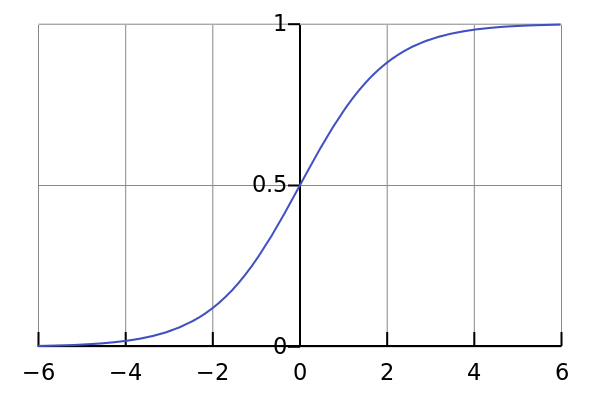
\includegraphics[width=9cm]{img/logistic.png}
	\caption{Graf logističke funkcije. }
	\label{fig:logistic}
\end{figure}
\end{frame}

\begin{frame}
\frametitle{Stroj potpornih vektora}
Stroj potpornih vektora jedan je od najpopularnijih modela strojnih učenja koji se danas koristi pri bilo kojoj klasifikaciji.
\bigskip

Stroj potpornih vektora na ulaz dobiva podatke povezane s klasom kojoj pripadaju te ih prikazuje kao točke u prostoru raspoređene na način da su točke koje predstavljaju podatke koji pripadaju različitim klasama međusobno što razmaknutije.
\bigskip

Zadatak stroja potpornog vektora je odabrati optimalnu hiperravninu razdvajanja.

\end{frame}

\begin{frame}
\frametitle{Odabir hiperravnine u stroju potpornih vektora.}
\begin{figure}[]
	\centering
	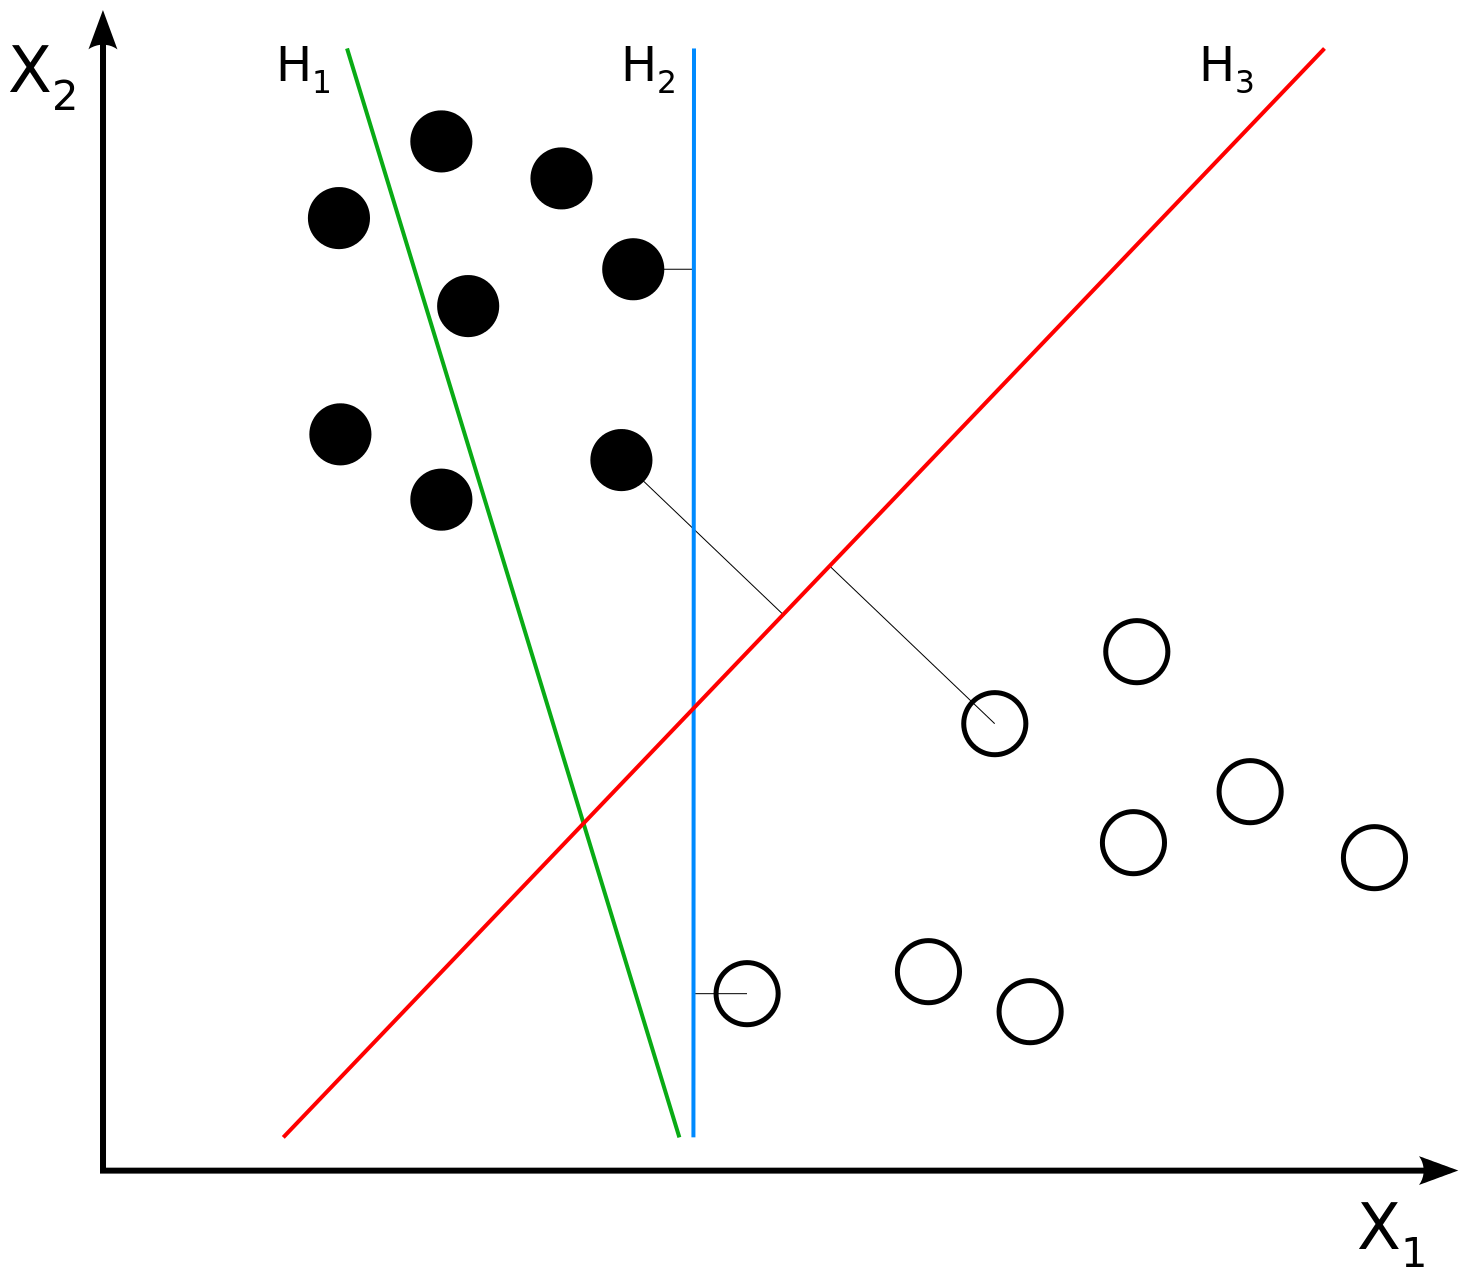
\includegraphics[width=7cm]{img/svm.png}
	\caption{Odabir hiperravnine u stroju potpornih vektora. }
	\label{fig:logistic}
\end{figure}
\end{frame}

\begin{frame}
\begin{center}
\Huge Podaci
\end{center}
\end{frame}

\begin{frame}
\frametitle{Prikupljanje podataka}
Podatke za ovaj rad prikupili smo s društvene mreže Reddit, s dretve naziva ``debateReligion".
\bigskip

Odabrali smo 4000 korisnika koji su raspravljali na spomenutoj dretvi te za svakog od njih su preuzeti svi komentari koje su ti korisnici ostavljali na društvenoj mreži Reddit, bez obzira o kojoj se dretvi radilo.

\end{frame}

\begin{frame}
\frametitle{Obrada podataka}
Obradu smo napravili u sljedećim koracima:

\begin{itemize}
\item Odbacivanje svih podatka koji nam nisu bitni za analizu
\item Spajanje svih komentara istog korisnika u jedan komentar
\item Standardizacija oznaka
\end{itemize}
\end{frame}

\begin{frame}
\frametitle{Model podataka}
Nakon obrade podataka u našim podatcima imamo 3733 redaka, svaki redak sadrži oznaku religije i tekst komentara.
\bigskip

U model podataka dodat ćemo frekvencije 700 najčešćih riječi koje se pojavljuju u svim komentarima nakon izbacivanja zaustavnih (engl.~\emph{stop}) riječi iz teksta.
\bigskip

U model podatka dodat ćemo i značajke LIWC koje smo dobili uz pomoć programa LIWC2015.

\end{frame}

\begin{frame}
\frametitle{Broj korisnika po religijama}
\begin{table}[h!]
\centering
\caption{Broj korisnika po religijama}
\label{table:dist}
\begin{tabular}{@{}ccc@{}}
\hline
Religija  & Broj korisnika & Postotak \\ 
\hline
\hline
Sekularni & 2228  &  59,68\%                 \\
Kršćani   & 567   & 15,18\%                 \\
Ostali    & 506  & 13,55\% \\
Bivši     & 208  & 5,57\%                   \\
Muslimani & 106  & 2,83\%                   \\
Židovi    & 63   & 1,69\%                  \\
Budisti   & 40   & 1,07\%                  \\
Hindusi   & 15  & 0,40\%                 \\
\hline
\end{tabular}
\end{table}

\end{frame}


\begin{frame}
\begin{center}
\Huge Rezultati
\end{center}
\end{frame}

\begin{frame}
\frametitle{Razlike u deskriptivnoj analizi}

\begin{table}[h!]
\small
\centering
\caption{Broj komentara po korisniku, broj riječi po komentaru i dužina riječi po religijama}
\label{table:desc}
\begin{tabular}{@{}cccc@{}}
\hline
Religija  & Broj komentara & Broj riječi po komentaru & Dužina riječi \\ 
\hline
\hline
Bivši     &  685,80   & 12,06                              & 5,39                    \\
Budisti   &  388,80    & 11,94                              & 5,35                    \\
Hindusi   &  617,40  & 11,82                              & 5,38                   \\
Kršćani   &  498,69   & 12,84                              & 5,38                    \\
Muslimani &  536,65  & 12,99                              & 5,37                    \\
Ostali    &  694,77    & 12,83                              & 5,50                    \\
Sekularni &  823,48  & 12,75                              & 5,38                    \\
Židovi    &  629,33  & 13,00                              & 5,41                    \\

\hline
\end{tabular}
\end{table}
\end{frame}


\begin{frame}
\frametitle{Razlike u vokabularu}
\begin{table}[h!]
\small
\centering
\caption{Deset najčešće korištenih riječi po religijama}
\label{table:voc}
\begin{tabular}{@{}cc@{}}
\hline
Religija  & Deset najčešće korištenih riječi                                       \\
\hline
\hline
Bivši     & \emph{people}, \emph{good}, \emph{will}, \emph{time}, \emph{well}, \emph{shit}, \emph{pretty}, \emph{thing}, \emph{going}, \emph{fuck}    \\
Budisti   & \emph{people}, \emph{will}, \emph{good}, \emph{time}, \emph{well}, \emph{sure}, \emph{pretty}, \emph{going}, \emph{better}, \emph{thing}  \\
Hindusi   & \emph{people}, \emph{will}, \emph{good}, \emph{india}, \emph{time}, \emph{well}, \emph{pretty}, \emph{better}, \emph{guy}, \emph{indian} \\
Kršćani   & \emph{people}, \emph{good}, \emph{will}, \emph{god}, \emph{time}, \emph{well}, \emph{going}, \emph{pretty}, \emph{sure}, \emph{thing}     \\
Muslimani & \emph{people}, \emph{will}, \emph{good}, \emph{islam}, \emph{time}, \emph{muslim}, \emph{muslims}, \emph{god}, \emph{well}, \emph{allah}  \\
Ostali    & \emph{people}, \emph{good}, \emph{will}, \emph{time}, \emph{well}, \emph{going}, \emph{thing}, \emph{better}, \emph{pretty}, \emph{watch} \\
Sekularni & \emph{people}, \emph{good}, \emph{will}, \emph{time}, \emph{well}, \emph{going}, \emph{thing}, \emph{pretty}, \emph{sure}, \emph{better}  \\
Židovi    & \emph{people}, \emph{jews}, \emph{will}, \emph{good}, \emph{jewish}, \emph{fine}, \emph{god}, \emph{israel}, \emph{thing}, \emph{going}   \\

\hline
\end{tabular}
\end{table}

\end{frame}


\begin{frame}
\frametitle{Razlike u značajkama LIWC}
\begin{table}[h!]
\small
\setlength{\tabcolsep}{2pt}
\centering
\caption{Tablica značajki LIWC}
\label{table:liwc}
\begin{tabular}{@{}cccccccc@{}}
\hline
Religija  & Religioznost & Uskličnici & Točka zarez & Obitelj & Hrana & Novac & Psovanje \\
\hline
\hline
Bivši     & 1,60         & 0,37       & 0,12        & 0,29    & 0,35  & 0,59  & 0,40     \\
Budisti   & 1,08         & 0,56       & 0,12        & 0,18    & 0,39  & 0,65  & 0,29     \\
Hindusi   & 2,13         & 0,25       & 0,09        & 0,21    & 0,23  & 0,42  & 0,32     \\
Kršćani   & 2,25         & 0,36       & 0,13        & 0,29    & 0,28  & 0,60  & 0,24     \\
Muslimani & 2,97         & 0,29       & 0,13        & 0,33    & 0,22  & 0,39  & 0,27     \\
Ostali    & 1,23         & 0,34       & 0,20        & 0,22    & 0,35  & 0,60  & 0,35     \\
Sekularni & 1,06         & 0,32       & 0,12        & 0,21    & 0,31  & 0,67  & 0,36     \\
Židovi    & 1,80         & 0,49       & 0,11        & 0,31    & 0,33  & 0,60  & 0,28     \\

\hline
\end{tabular}
\end{table}
\end{frame}


\begin{frame}
\frametitle{Zaključci inferencijalne analize}
\begin{table}[h!]
\small
\centering
\caption{Rezultati testne statistike}
\label{table:inf}
\begin{tabular}{@{}cc@{}}
\hline
Značajka             & Vrijednost testne statistike   \\ 
\hline
\hline
Frekvencija ``muslim" & 2*10\textasciicircum{}-16    \\
Frekvencija ``jews"   & 2*10\textasciicircum{}-16    \\
Frekvencija ``shit"   & 1,5*10\textasciicircum{}-8   \\
LIWC ``Religioznost"  & 2*10\textasciicircum{}-16    \\
LIWC ``Uskličnici"    & 0,000587                     \\
LIWC ``Točka zarez"   & 0,00195                      \\
LIWC ``Obitelj"       & 2*10\textasciicircum{}-16    \\
LIWC ``Hrana"         & 1,02*10\textasciicircum{}-6  \\ 
LIWC ``Novac"         & 5,21*10\textasciicircum{}-12 \\
LIWC ``Psovanje"      & 3,22*10\textasciicircum{}-16 \\ 
\hline
\end{tabular}
\end{table}
\end{frame}

\begin{frame}
\frametitle{Predikcije logističke regresije}

\begin{table}[h!]
\centering
\caption{Rezultati na skupu za treniranje}
\label{table:logTrain}
\begin{tabular}{@{}ccccc@{}}
\hline
Pogodak & Promašaj & Točnost  & 95\%-tni interval pouzdanosti \\
\hline
\hline
2012     & 988      & 67,07\% & 67,04\%-67,10\%  \\
\hline
\end{tabular}
\end{table}


\begin{table}[h!]
\centering
\caption{Rezultati na skupu za testiranje}
\label{table:logTest}
\begin{tabular}{@{}ccccc@{}}
\hline
Pogodak & Promašaj & Točnost  & 95\%-tni interval pouzdanosti\\
\hline
\hline
457     & 276      & 62,36\% & 62,30\%-62,43\% \\
\hline
\end{tabular}
\end{table}

\end{frame}


\begin{frame}
\frametitle{Predikcije stroja potpornih vektora}

\begin{table}[h!]
\centering
\caption{Rezultati na skupu za treniranje}
\label{table:svmTrain}
\begin{tabular}{@{}ccccc@{}}
\hline
Pogodak & Promašaj & Točnost  &  95\%-tni interval pouzdanosti\\
\hline
\hline
2077     & 923      & 69,23\% & 69,20\%-69,27\% \\
\hline
\end{tabular}
\end{table}



\begin{table}[h!]
\centering
\caption{Rezultati na skupu za testiranje}
\label{table:svmTest}
\begin{tabular}{@{}ccccc@{}}
\hline
Pogodak & Promašaj & Točnost  &  95\%-tni interval pouzdanosti\\
\hline
\hline
473     & 260      & 64,53\% & 64,46\%-64,59\% \\
\hline
\end{tabular}
\end{table}

\end{frame}


\begin{frame}
\frametitle{Zaključak}
Glavna motivacija ovog rada je bila vidjeti postoje li razlike u internetskim raspravama između religija. 
\bigskip

Uspjeli smo statistički uvidjeti da postoje razlike u načinu izražavanja na internetu između religija.
\bigskip

U ovom radu uspješno smo izgradili model koji s točnošću od otprilike 65\% predviđa koje je religijske orijentacije korisnik koji je napisao komentare.
\bigskip

Rezultati dobiveni u ovom radu, otvaraju daljnje mogućnosti istraživanja međureligijskih odnosa i razlika. 
\bigskip

Osim statistički, ovaj problem bi se sigurno trebao sagledati s teološke i psihološke perspektive, pogotovo nakon što nam je statistika pokazala da razlike postoje.



\end{frame}

\begin{frame}
\begin{center}
\Huge Hvala na pažnji! Pitanja?
\end{center}
\end{frame}
 
\end{document}
